%(BEGIN_QUESTION)
% Copyright 2009, Tony R. Kuphaldt, released under the Creative Commons Attribution License (v 1.0)
% This means you may do almost anything with this work of mine, so long as you give me proper credit

An NDIR gas analyzer is going to be used to measure the percentage balance between methane (CH$_{4}$) gas and ethane (C$_{2}$H$_{6}$) gas in a process stream where {\it only} these two hydrocarbon gases exist, and the mixture is approximately half-and-half.  The infrared absorption characteristics of both gases are shown in the following plot (methane in blue; ethane in red):

$$\includegraphics[width=15.5cm]{i04176x01.eps}$$

Identify which gases the ``reference cell'' and ``detector'' chambers should be filled with, and whether or not this analyzer will require filter cells.  If filter cells are required, identify the gas(es) they should be filled with as well.

Also, identify whether it matters which of these two gases the analyzer is ``sensitized'' to, since the percentage balance between methane and ethane in this process stream is nearly 50\%-50\%.

\vskip 20pt \vbox{\hrule \hbox{\strut \vrule{} {\bf Suggestions for Socratic discussion} \vrule} \hrule}

\begin{itemize}
\item{} If this sample stream were analyzed by a gas chromatograph, which compound peak would appear {\it first} on the chromatogram, methane or ethane?
\item{} Describe a full calibration procedure for this analyzer, by which you may check its LRV, URV, and also check to see that the interfering gas has negligible effect.
\end{itemize}

\underbar{file i04176}
%(END_QUESTION)





%(BEGIN_ANSWER)

\noindent
{\bf Partial answer:}

\vskip 10pt

Filter cells {\it are required} for this NDIR analyzer, and they {\it must} be filled with ethane gas!

%(END_ANSWER)





%(BEGIN_NOTES)

Fill the detector chambers with methane gas.  Fill the reference cell with any non-absorbing gas (e.g. nitrogen).  Fill the filter cells with ethane gas.

\vskip 10pt

This analyzer will not function for this process if sensitized for ethane (i.e. ethane gas in the Luft detector, methane in the filter cells), because the methane gas in the filter cells will practically eliminate all ethane response.  Ethane has no IR absorption outside of those regions dominated by methane, which means methane filtering will eliminate all absorption by ethane.  However, since methane {\it does} have absorption bands outside of ethane's, it makes sense to filter for ethane and sensitize for methane.

%INDEX% Measurement, analytical: nondispersive optical

%(END_NOTES)


